%%PREAMBLE %%%%%%%%%%%%%%%%%%%%%%%%%%%%
\documentclass[10pt, a4paper]{article}% size of txt = 10pt
\usepackage[top= 2cm,
			bottom = 2cm,
			left = 1.7cm,
			right = 1.7cm,
			footskip = 0.5cm,
			headsep = 0cm,
			headheight = 0cm
					]{geometry}
\usepackage{amsmath} % math packages
\usepackage{amsfonts}% math packages
\usepackage{amssymb} % math packages
\usepackage{graphicx} %package for including graphics
\usepackage{array}
\usepackage[thinlines]{easytable}
\usepackage{float}
\usepackage[section]{placeins}
\usepackage[hidelinks]{hyperref}
\usepackage[shortlabels]{enumitem}
\usepackage{svg}
\usepackage{bigstrut}
\usepackage{wrapfig,lipsum,booktabs}
\usepackage{subcaption}
\usepackage{xfrac}
\usepackage{pdfpages}
\usepackage{listings}
\usepackage{xcolor}

\usepackage{listings}
\usepackage{color} %red, green, blue, yellow, cyan, magenta, black, white
\definecolor{mygreen}{RGB}{28,172,0} % color values Red, Green, Blue
\definecolor{mylilas}{RGB}{170,55,241}

\definecolor{codegreen}{rgb}{0,0.6,0}
\definecolor{codegray}{rgb}{0.5,0.5,0.5}
\definecolor{codepurple}{rgb}{0.58,0,0.82}
\definecolor{backcolour}{rgb}{1,1,1}

\lstdefinestyle{mystyle}{
    backgroundcolor=\color{backcolour},   
    commentstyle=\color{codegreen},
    keywordstyle=\color{magenta},
    numberstyle=\tiny\color{codegray},
    stringstyle=\color{codepurple},
    basicstyle=\ttfamily\footnotesize,
    breakatwhitespace=false,         
    breaklines=true,                 
    captionpos=b,                    
    keepspaces=true,                 
    numbers=left,                    
    numbersep=5pt,                  
    showspaces=false,                
    showstringspaces=false,
    showtabs=false,                  
    tabsize=2
}
\lstset{style=mystyle}


%date format
\def\mydate{\leavevmode\hbox{\twodigits\day.\twodigits\month.\the\year}}
\def\twodigits#1{\ifnum#1<10 0\fi\the#1}


\usepackage[T1]{fontenc} 
\usepackage{lmodern}
\usepackage{indentfirst}
\setlength{\parindent}{1cm}

\makeatletter
\newcommand{\thickhline}{%
    \noalign {\ifnum 0=`}\fi \hrule height 2pt
    \futurelet \reserved@a \@xhline
}
\newcolumntype{"}{@{\hskip\tabcolsep\vrule width 2pt\hskip\tabcolsep}}
\makeatother
\newcolumntype{?}{!{\vrule width 2pt}}
%%DOC ENVIROMENT%%%%%%%%%%%%%%%%%%%%%%%
\begin{document}
%Title 
\begin{flushleft}%% left justification
	\textbf{\Large{MKC-DVV: Laboratorní úloha č.6}}\hfill Filip Paul\\
	\large{Měření parametrů signálu při příjmu DAB/DAB+ \hfill\mydate}

\end{flushleft}
\section{\Large Výsledky měření:}
\noindent Vzhledem k tomu, že výsledný protokol obsahuje fotografie ze 2 laboratorních cvičení a jeho velikost překračuje 5MB.
Přidávám odkaz na protokol ve verzi s fotkama, kterou si můžete stáhnout z mého github repozitáře zde:
\href{https://github.com/FilipPaul/PATAK_zimni/blob/main/DVV/LAB6/DVV_LAB_2a6_PAUL.pdf}{\color{blue}PDF final}


\noindent Tento dokument je verzí bez fotografií !!!\\ 

Z níže naměřených hodnot je patrné, že s zlepšujícím se C/N se zlepšuje i SNR, což odpovídá teoretickým předpokladům. Zajímavé však je, pro
nízké C/N (přibližně do C/N = 15) nemá téměř žádný význam zvyšovat výkon vysílače, protože zlepšení SNR je minimální. Zvláštní však je, že
pro určité hodnoty C/N, vyšlo naměřené SNR lepší pro výstupní výkon vysílače -50dBm než pro -20dBm. Tuto zvláštnost přisuzuji
především nesprávnému odečtu SNR z ovládacího softwaru pro DAB radio, protože hodnoty SNR během měření nebyly stabilní. Ručně nakreslená spektra
společně s podpisem jsou na konci tohoto dokumentu.
\begin{table}[ht!]
    \begin{minipage}{0.5\textwidth}
    \resizebox{!}{!}{%
    \begin{tabular}{|cccc|}
    \hline
    \multicolumn{4}{|c|}{\textbf{závislost SNR na C/N pro P = -20, -50 a -70 dBm}}                                                             \\ \hline
    \multicolumn{1}{|c|}{\textbf{C/N : P}} & \multicolumn{1}{c|}{\textbf{-70 dBm}} & \multicolumn{1}{c|}{\textbf{-50 dBm}} & \textbf{-20 dBm} \\ \hline
    \multicolumn{1}{|c|}{\textbf{40}}      & \multicolumn{1}{c|}{25,4}            & \multicolumn{1}{c|}{33,5}            & 31,9            \\ \hline
    \multicolumn{1}{|c|}{\textbf{35}}      & \multicolumn{1}{c|}{25,8}            & \multicolumn{1}{c|}{31,4}            & 31,8            \\ \hline
    \multicolumn{1}{|c|}{\textbf{30}}      & \multicolumn{1}{c|}{25,2}            & \multicolumn{1}{c|}{30,7}            & 29,6            \\ \hline
    \multicolumn{1}{|c|}{\textbf{25}}      & \multicolumn{1}{c|}{24,4}            & \multicolumn{1}{c|}{27,5}            & 26,4            \\ \hline
    \multicolumn{1}{|c|}{\textbf{20}}      & \multicolumn{1}{c|}{22,6}            & \multicolumn{1}{c|}{24,4}            & 24,1            \\ \hline
    \multicolumn{1}{|c|}{\textbf{17}}      & \multicolumn{1}{c|}{20,5}            & \multicolumn{1}{c|}{21,4}            & 21,3            \\ \hline
    \multicolumn{1}{|c|}{\textbf{15}}      & \multicolumn{1}{c|}{19,2}            & \multicolumn{1}{c|}{20,1}            & 19,7            \\ \hline
    \multicolumn{1}{|c|}{\textbf{12}}      & \multicolumn{1}{c|}{16,6}            & \multicolumn{1}{c|}{17,1}            & 17,2            \\ \hline
    \multicolumn{1}{|c|}{\textbf{10}}      & \multicolumn{1}{c|}{14,7}            & \multicolumn{1}{c|}{15,1}            & 15,2            \\ \hline
    \multicolumn{1}{|c|}{\textbf{5}}       & \multicolumn{1}{c|}{10,2}            & \multicolumn{1}{c|}{10,4}            & 10,4            \\ \hline
    \multicolumn{1}{|c|}{\textbf{3}}       & \multicolumn{1}{c|}{8,5}             & \multicolumn{1}{c|}{8,5}             & 8,5             \\ \hline
    \multicolumn{1}{|c|}{\textbf{0}}       & \multicolumn{1}{c|}{6}               & \multicolumn{1}{c|}{6,1}             & 6               \\ \hline
    \end{tabular}%
    }
\end{minipage}
\hfill
\begin{minipage}{0.45\textwidth}
    \centering
    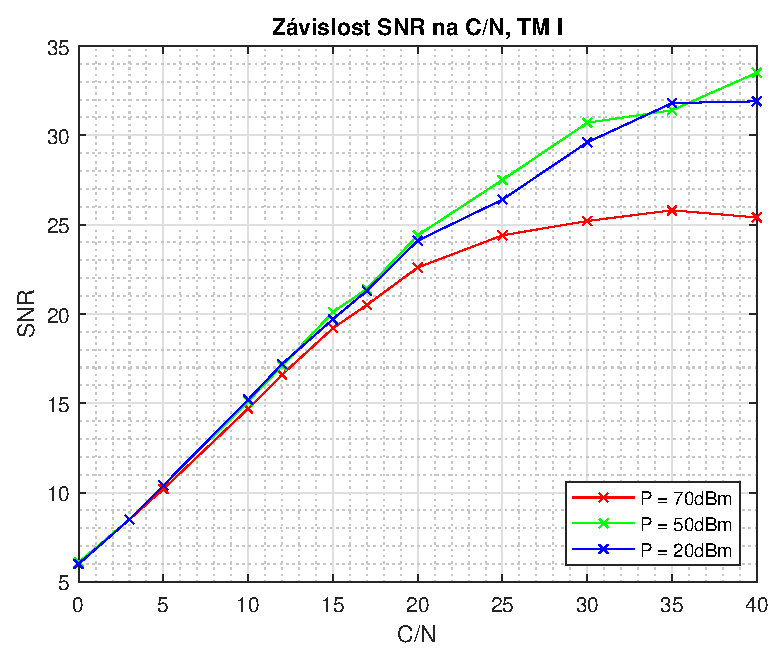
\includegraphics[width=1\textwidth]{SNR_CN.eps}
\end{minipage}

\end{table}


Následující změřené hodnoty odpovídají opět závislosti SNR na C/N. Nicméně tentokrát jsou všechny hodnoty změřeny pro výstupní výkon -50dBm
a mění se vysílací módy (TM II, III a IV). Z naměřených hodnot vychází nejlepší SNR pro mód TM III. Nicméně i tomto měření bylo 
prováděno odečítání hodnot SNR s poměrně značnou chybou, protože hodnoty SNR nebyly stabilní.
\begin{table}[ht!]
    \begin{minipage}{0.5\textwidth}
    \resizebox{!}{!}{%
    \begin{tabular}{|ccccc|}
        \hline
        \multicolumn{5}{|c|}{\textbf{Závislost SNR na C/N pro TM = II, III a IV}}                                        \\ \hline
        \multicolumn{1}{|c|}{\textbf{CN : TM}} & \multicolumn{1}{c|}{\textbf{I}} & \multicolumn{1}{c|}{\textbf{II}} & \multicolumn{1}{c|}{\textbf{III}} & \textbf{IV} \\ \hline
        \multicolumn{1}{|c|}{\textbf{40}} & \multicolumn{1}{c|}{33,5} & \multicolumn{1}{c|}{32,2} & \multicolumn{1}{c|}{32,4} & 32,2 \\ \hline
        \multicolumn{1}{|c|}{\textbf{35}} & \multicolumn{1}{c|}{31,4} & \multicolumn{1}{c|}{31,2} & \multicolumn{1}{c|}{32,5} & 29,7 \\ \hline
        \multicolumn{1}{|c|}{\textbf{30}} & \multicolumn{1}{c|}{30,7} & \multicolumn{1}{c|}{30,5} & \multicolumn{1}{c|}{30,6} & 28,6 \\ \hline
        \multicolumn{1}{|c|}{\textbf{25}} & \multicolumn{1}{c|}{27,5} & \multicolumn{1}{c|}{27,5} & \multicolumn{1}{c|}{28,2} & 26,4 \\ \hline
        \multicolumn{1}{|c|}{\textbf{20}} & \multicolumn{1}{c|}{24,4} & \multicolumn{1}{c|}{24,4} & \multicolumn{1}{c|}{24,4} & 23,5 \\ \hline
        \multicolumn{1}{|c|}{\textbf{17}} & \multicolumn{1}{c|}{21,4} & \multicolumn{1}{c|}{22}   & \multicolumn{1}{c|}{21,8} & 21,4 \\ \hline
        \multicolumn{1}{|c|}{\textbf{15}} & \multicolumn{1}{c|}{20,1} & \multicolumn{1}{c|}{19,8} & \multicolumn{1}{c|}{20,1} & 20   \\ \hline
        \multicolumn{1}{|c|}{\textbf{12}} & \multicolumn{1}{c|}{17,1} & \multicolumn{1}{c|}{16,9} & \multicolumn{1}{c|}{17,4} & 16,8 \\ \hline
        \multicolumn{1}{|c|}{\textbf{10}} & \multicolumn{1}{c|}{15,1} & \multicolumn{1}{c|}{15,2} & \multicolumn{1}{c|}{15}   & 15,2 \\ \hline
        \multicolumn{1}{|c|}{\textbf{5}}  & \multicolumn{1}{c|}{10,4} & \multicolumn{1}{c|}{10,4} & \multicolumn{1}{c|}{10,9} & 10,2 \\ \hline
        \multicolumn{1}{|c|}{\textbf{3}}  & \multicolumn{1}{c|}{8,5}  & \multicolumn{1}{c|}{8,5}  & \multicolumn{1}{c|}{8,2}  & 8,8  \\ \hline
        \multicolumn{1}{|c|}{\textbf{0}}  & \multicolumn{1}{c|}{6,1}  & \multicolumn{1}{c|}{6,1}  & \multicolumn{1}{c|}{6,1}  & 5,8  \\ \hline
        \end{tabular}%
    }
\end{minipage}
\hfill
\begin{minipage}{0.45\textwidth}
    \centering
    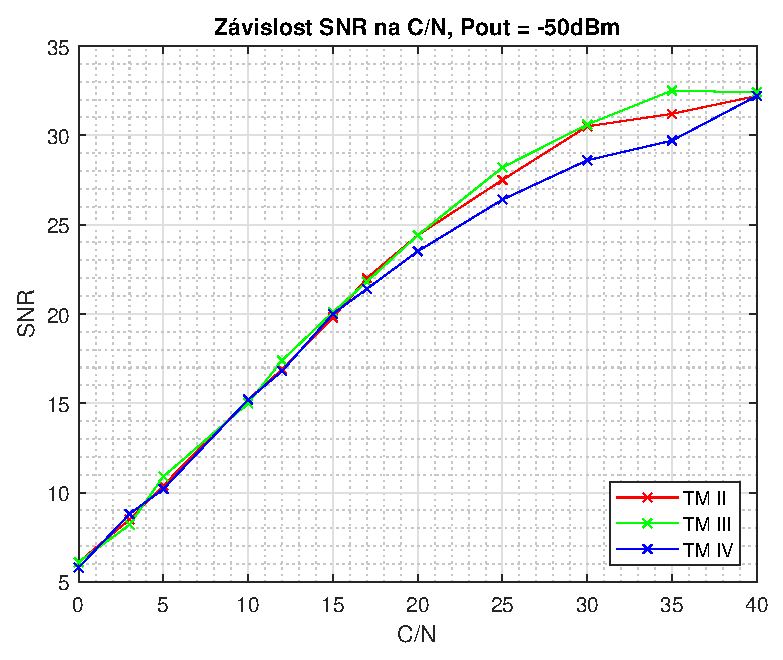
\includegraphics[width=1\textwidth]{SNR_CN_TM_MODES.eps}
\end{minipage}

\end{table}


\clearpage
Poslední měření se zabývá vlivem únikových kanálů (RA6,RA12, TU6 a TU12) na výsledné SNR. Únikové kanály RA simulují pohyb přijímače ve venkovské
oblasti rychlostí 100 km/h. TU pak pohyb přijímače v městských oblastech rychlostí 50 km/h. Vzhledem k tomu, že při tomto měření SNR
probíhalo odečítání SNR hodnot pomocí aproximace od oka.. Z důvodu rozkmitu SNR řádově $\pm$10dB jsou výsledky k dalšímu komentáři značně
spekulativní. Pokud však budeme výsledkům věřit, lze usoudit, že vysílaní DAB je odolnější proti únikovému kanálu TU.
\begin{table}[ht!]
    \begin{minipage}{0.5\textwidth}
    \resizebox{!}{!}{%
    \begin{tabular}{|ccccc|}
        \hline
        \multicolumn{5}{|c|}{\textbf{Závislost SNR na C/N pro únikové kanály}}                                                                                          \\ \hline
        \multicolumn{1}{|c|}{\textbf{CN: FADE}} &
          \multicolumn{1}{c|}{\textbf{RA 4}} &
          \multicolumn{1}{c|}{\textbf{RA 6}} &
          \multicolumn{1}{c|}{\textbf{TU 6}} &
          \textbf{TU 12} \\ \hline
        \multicolumn{1}{|c|}{\textbf{40}} & \multicolumn{1}{c|}{21,8} & \multicolumn{1}{c|}{32,7} & \multicolumn{1}{c|}{29,1} & 27,7 \\ \hline
        \multicolumn{1}{|c|}{\textbf{35}} & \multicolumn{1}{c|}{19,7} & \multicolumn{1}{c|}{29,1} & \multicolumn{1}{c|}{25,5} & 26,4 \\ \hline
        \multicolumn{1}{|c|}{\textbf{30}} & \multicolumn{1}{c|}{15,5} & \multicolumn{1}{c|}{28,1} & \multicolumn{1}{c|}{26,4} & 26,2 \\ \hline
        \multicolumn{1}{|c|}{\textbf{25}} & \multicolumn{1}{c|}{13,5} & \multicolumn{1}{c|}{20}   & \multicolumn{1}{c|}{24,7} & 24,6 \\ \hline
        \multicolumn{1}{|c|}{\textbf{20}} & \multicolumn{1}{c|}{12,6} & \multicolumn{1}{c|}{14,3} & \multicolumn{1}{c|}{21,7} & 21,5 \\ \hline
        \multicolumn{1}{|c|}{\textbf{17}} & \multicolumn{1}{c|}{10,2} & \multicolumn{1}{c|}{14,1} & \multicolumn{1}{c|}{19,2} & 19   \\ \hline
        \multicolumn{1}{|c|}{\textbf{15}} & \multicolumn{1}{c|}{11}   & \multicolumn{1}{c|}{15}   & \multicolumn{1}{c|}{17,3} & 17   \\ \hline
        \multicolumn{1}{|c|}{\textbf{10}} & \multicolumn{1}{c|}{8,4}  & \multicolumn{1}{c|}{10,6} & \multicolumn{1}{c|}{13,7} & 14,9 \\ \hline
        \multicolumn{1}{|c|}{\textbf{5}}  & \multicolumn{1}{c|}{5,5}  & \multicolumn{1}{c|}{7}    & \multicolumn{1}{c|}{9,8}  & 11,3 \\ \hline
        \multicolumn{1}{|c|}{\textbf{0}}  & \multicolumn{1}{c|}{2,7}  & \multicolumn{1}{c|}{3,5}  & \multicolumn{1}{c|}{4,8}  & 5,4  \\ \hline
        \end{tabular}%
    }
\end{minipage}
\hfill
\begin{minipage}{0.45\textwidth}
    \centering
    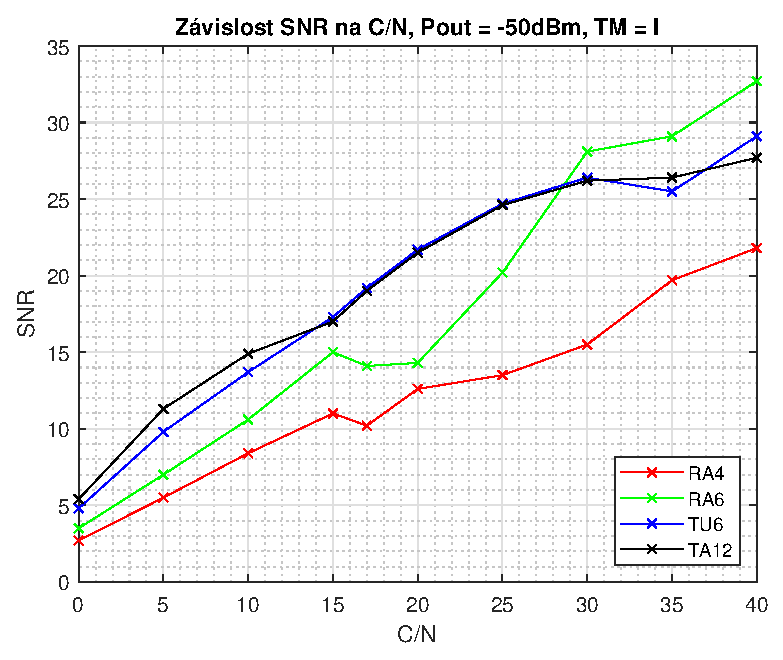
\includegraphics[width=1\textwidth]{SNR_CN_CHANNELS.eps}
\end{minipage}

\end{table}


\section{\Large Přijaté DAB vysílání:}
Celkově bylo přijato 17 DAB vysílání. Následující obrázky zachycují seznam přijatých stanic a servisní informace
pro vybrané DAB vysílání.
%\begin{figure}[ht!]
%    \begin{minipage}{0.5\textwidth}
%        \centering
%        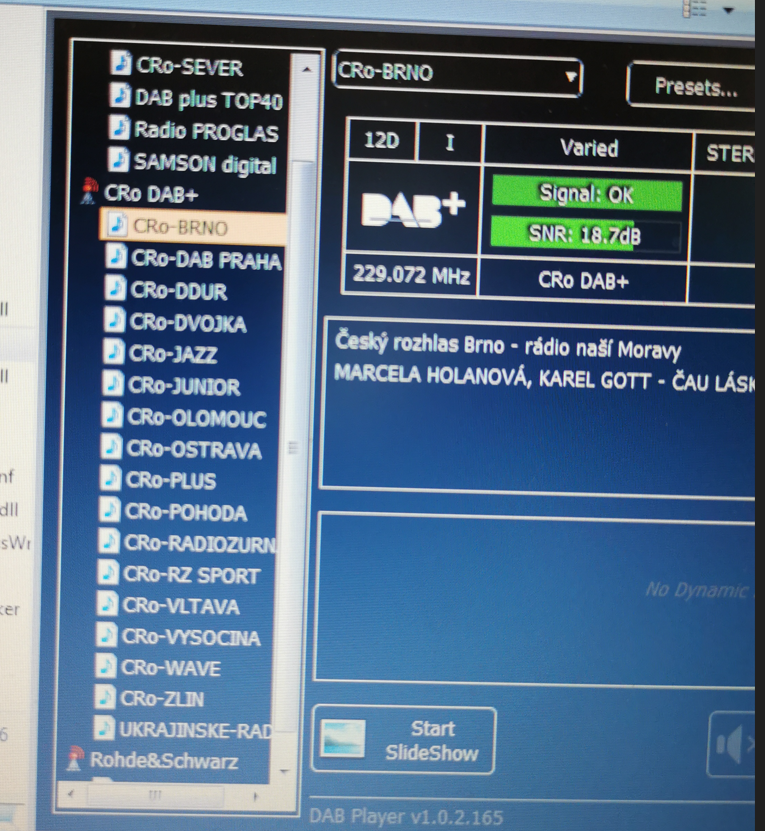
\includegraphics[height = 0.2\textheight]{all_radios.png}
%        \caption{Všechny přijaté DAB vysílání (17 stanic)}
%    \end{minipage}
%    \begin{minipage}{0.5\textwidth}
%        \centering
%        \includegraphics[height = 0.2\textheight]{CRO_BRNO.jpg}
%        \caption{Servisní informace CRO Brno}
%    \end{minipage}
%    \begin{minipage}{0.5\textwidth}
%        \centering
%        \includegraphics[height = 0.2\textheight]{CRO_DAB_PRAHA.jpg}
%        \caption{Servisní informace CRO Praha}
%    \end{minipage}
%    \begin{minipage}{0.5\textwidth}
%        \centering
%        \includegraphics[height = 0.2\textheight]{CRO_DVOJKA.jpg}
%        \caption{Servisní informace CRO Dvojka}
%    \end{minipage}
%    
%\end{figure}


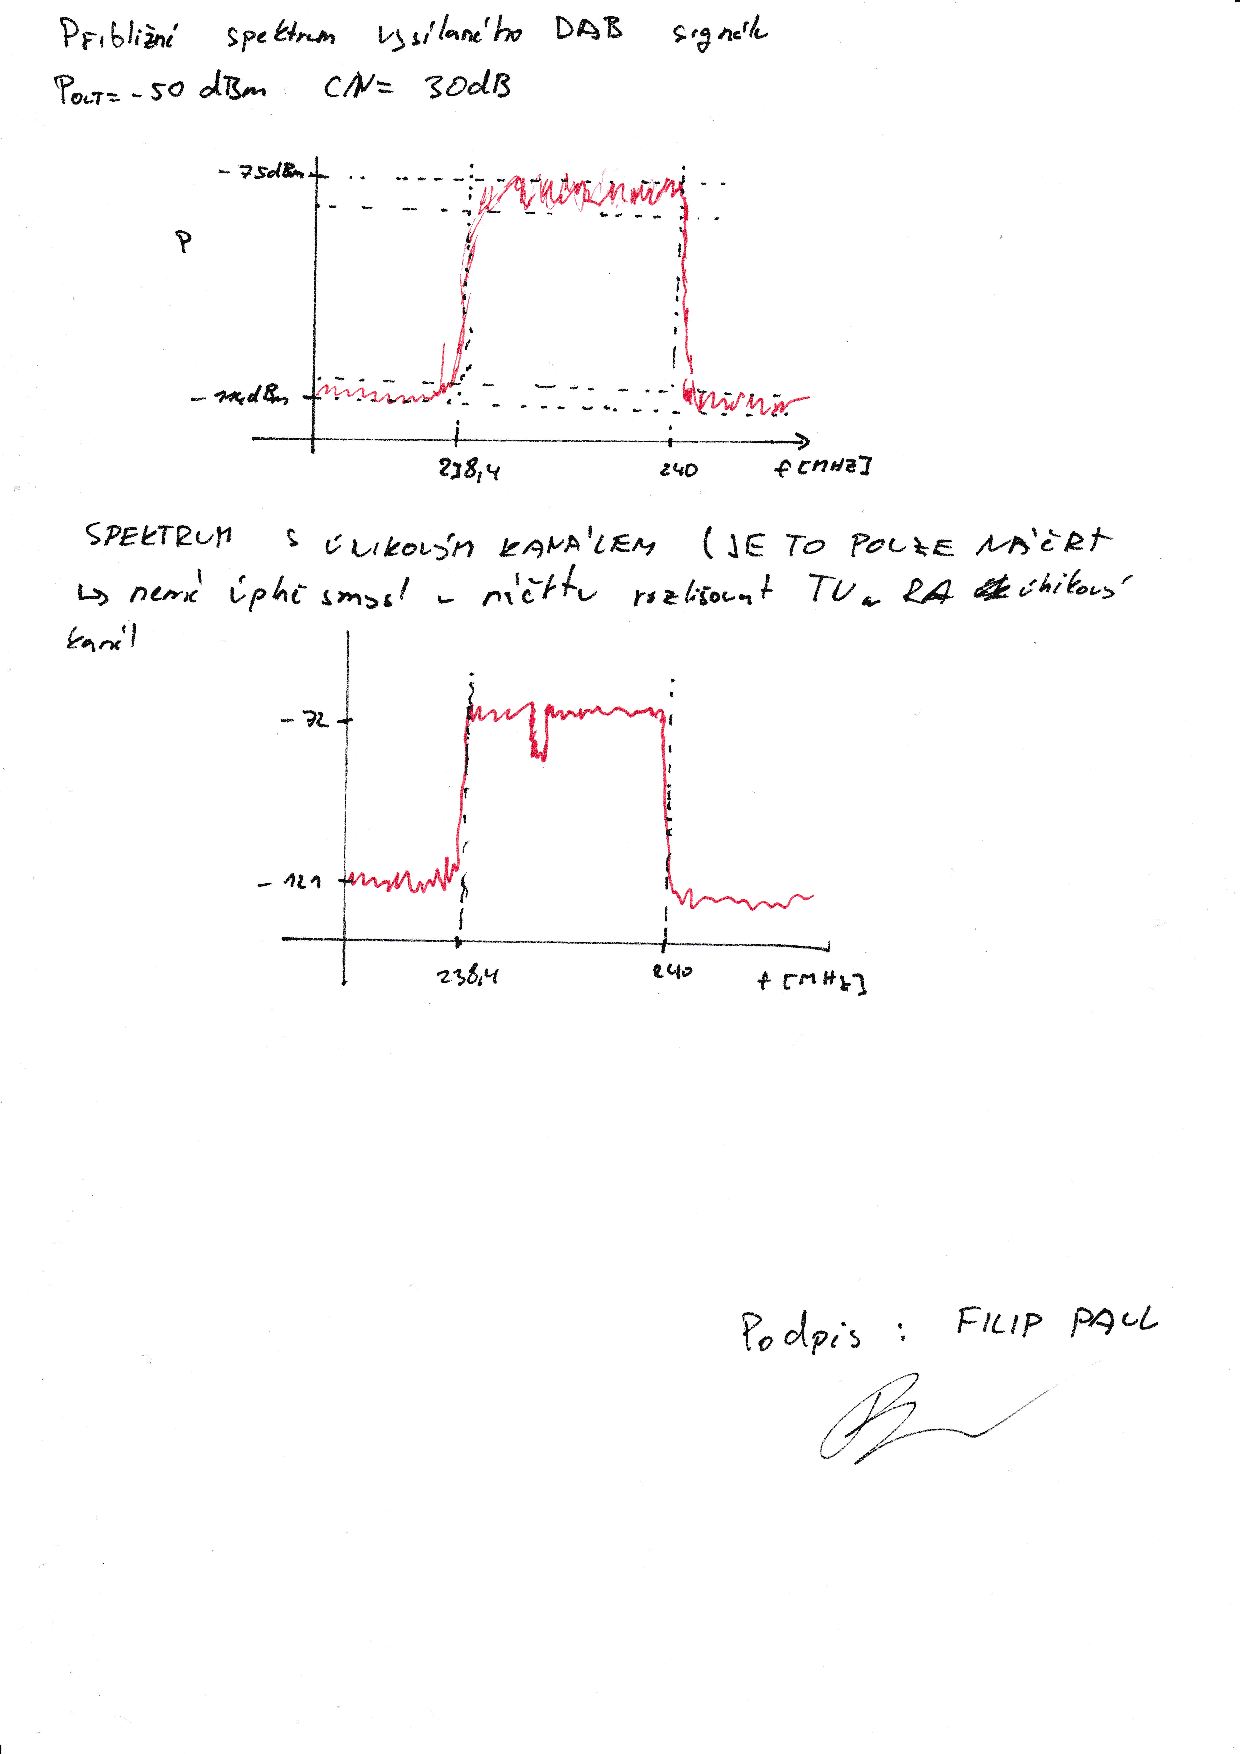
\includepdf{DVV_lab6_podpis.pdf}
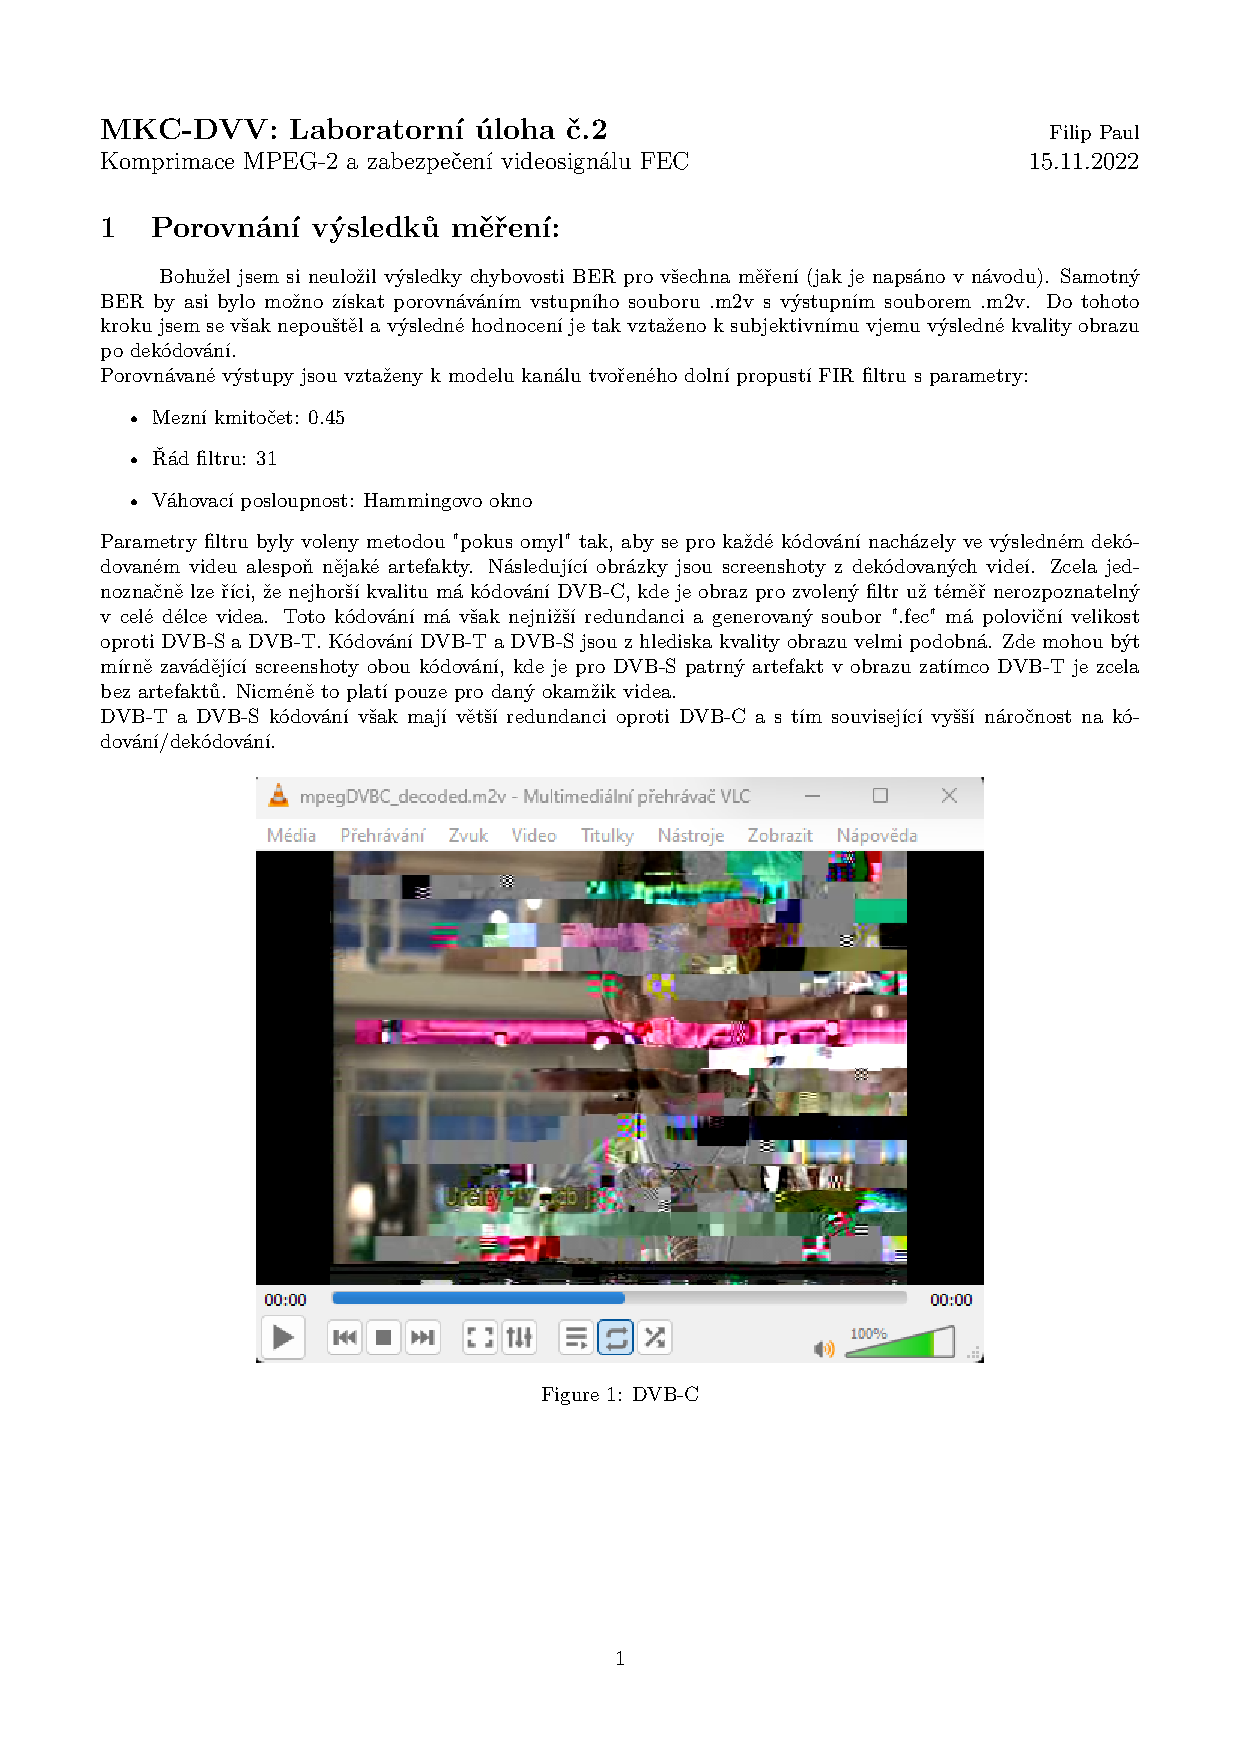
\includepdf[pages={1-}]{../LAB2/DVV_LAB2_PAUL.pdf}
\end{document}

%\[f(x)= (x+2)^2 - \frac{9\cdot 2\pi}{26}\] %%mathematic equatation in display style mode
%%optional:
%	\begin{align} %%this alignes all charakters after & if *is removed equations will be numbered
%	\hspace{5cm}  
%		 x &= a_2 x^2 +_1 x + a_0 \\
% 		x &=x^2 \nonumber		%no number will not add number to eq
%	\end{align}


